\section{Results}
\label{sec:analysis}
\label{sec:results}
This section contains the methodological results and the analyses of the selected articles. We first report study selection and the validation of screening and extraction, then the characteristics of the \edit{115} included studies: publication trends, modalities and territories, tasks and architectures, temporal modeling, venues, reported performance and reporting quality.

\subsection{Study Selection and Review Corpus}
The screening search identified 5,829 records (PubMed/\allowbreak MEDLINE 4,071; Semantic Scholar 1,758). After removing 765 duplicates, 5,064 records remained. The LLM \edit{labeled} 134 as eligible and excluded 4,930. 4,831 failed at least one inclusion criterion and 99 met an exclusion criterion (E1: 3, E2: 95, E3: 1). The PRISMA diagram of this eligibility analysis is shown in Figure~\ref{fig:prisma}.

Applying Cochran's \cite{cochran1977sampling} formula, we set the validation sample at 357 of the 4,930 exclusions; we also included all the LLM-eligible articles, which resulted in 491 records for manual review.

The two reviewers agreed on 487 of the 491 records (99.2\%; Cohen's $\kappa=0.978$, 95\% CI 0.957--0.999). The four cases with disagreements were resolved through discussion by the annotators. The resultant data, after resolution of the disagreements, served as the manually validated dataset.

The manually validated dataset contained 122 eligible reports (14 LLM-eligible records were excluded, while 2 LLM-non-eligible records were added) for review. Full text could not be retrieved for 2 of \edit{these, so 120 reports were assessed at full text. During full text analysis, we found that two of them were published meeting abstracts without a full methods section, so they were excluded under E1. Of} the \edit{remaining} \edit{118 reports, three were earlier versions (two preprints and one conference paper) of an included journal article; we counted each study once, using} the \edit{journal version. The} final review corpus \edit{therefore} comprises \edit{115} studies. 

% All 491 screening decisions are listed in Supplementary Table~S1.


The full-text LLM extraction audit covered 6 of the \edit{115} studies (5\%) and 444 values. Each study contained 74 fields: 18 study-level fields, the status of the 12 research gaps, and 44 CLAIM-informed reporting criteria. Disagreements were resolved through discussion to obtain the final validated set. Inter-annotator agreement was \(\kappa = 0.967\). Compared with the validated set, 431 of 444 extracted values were correct (97.1\%).




\begin{figure*}[pos=htbp]
  \centering
  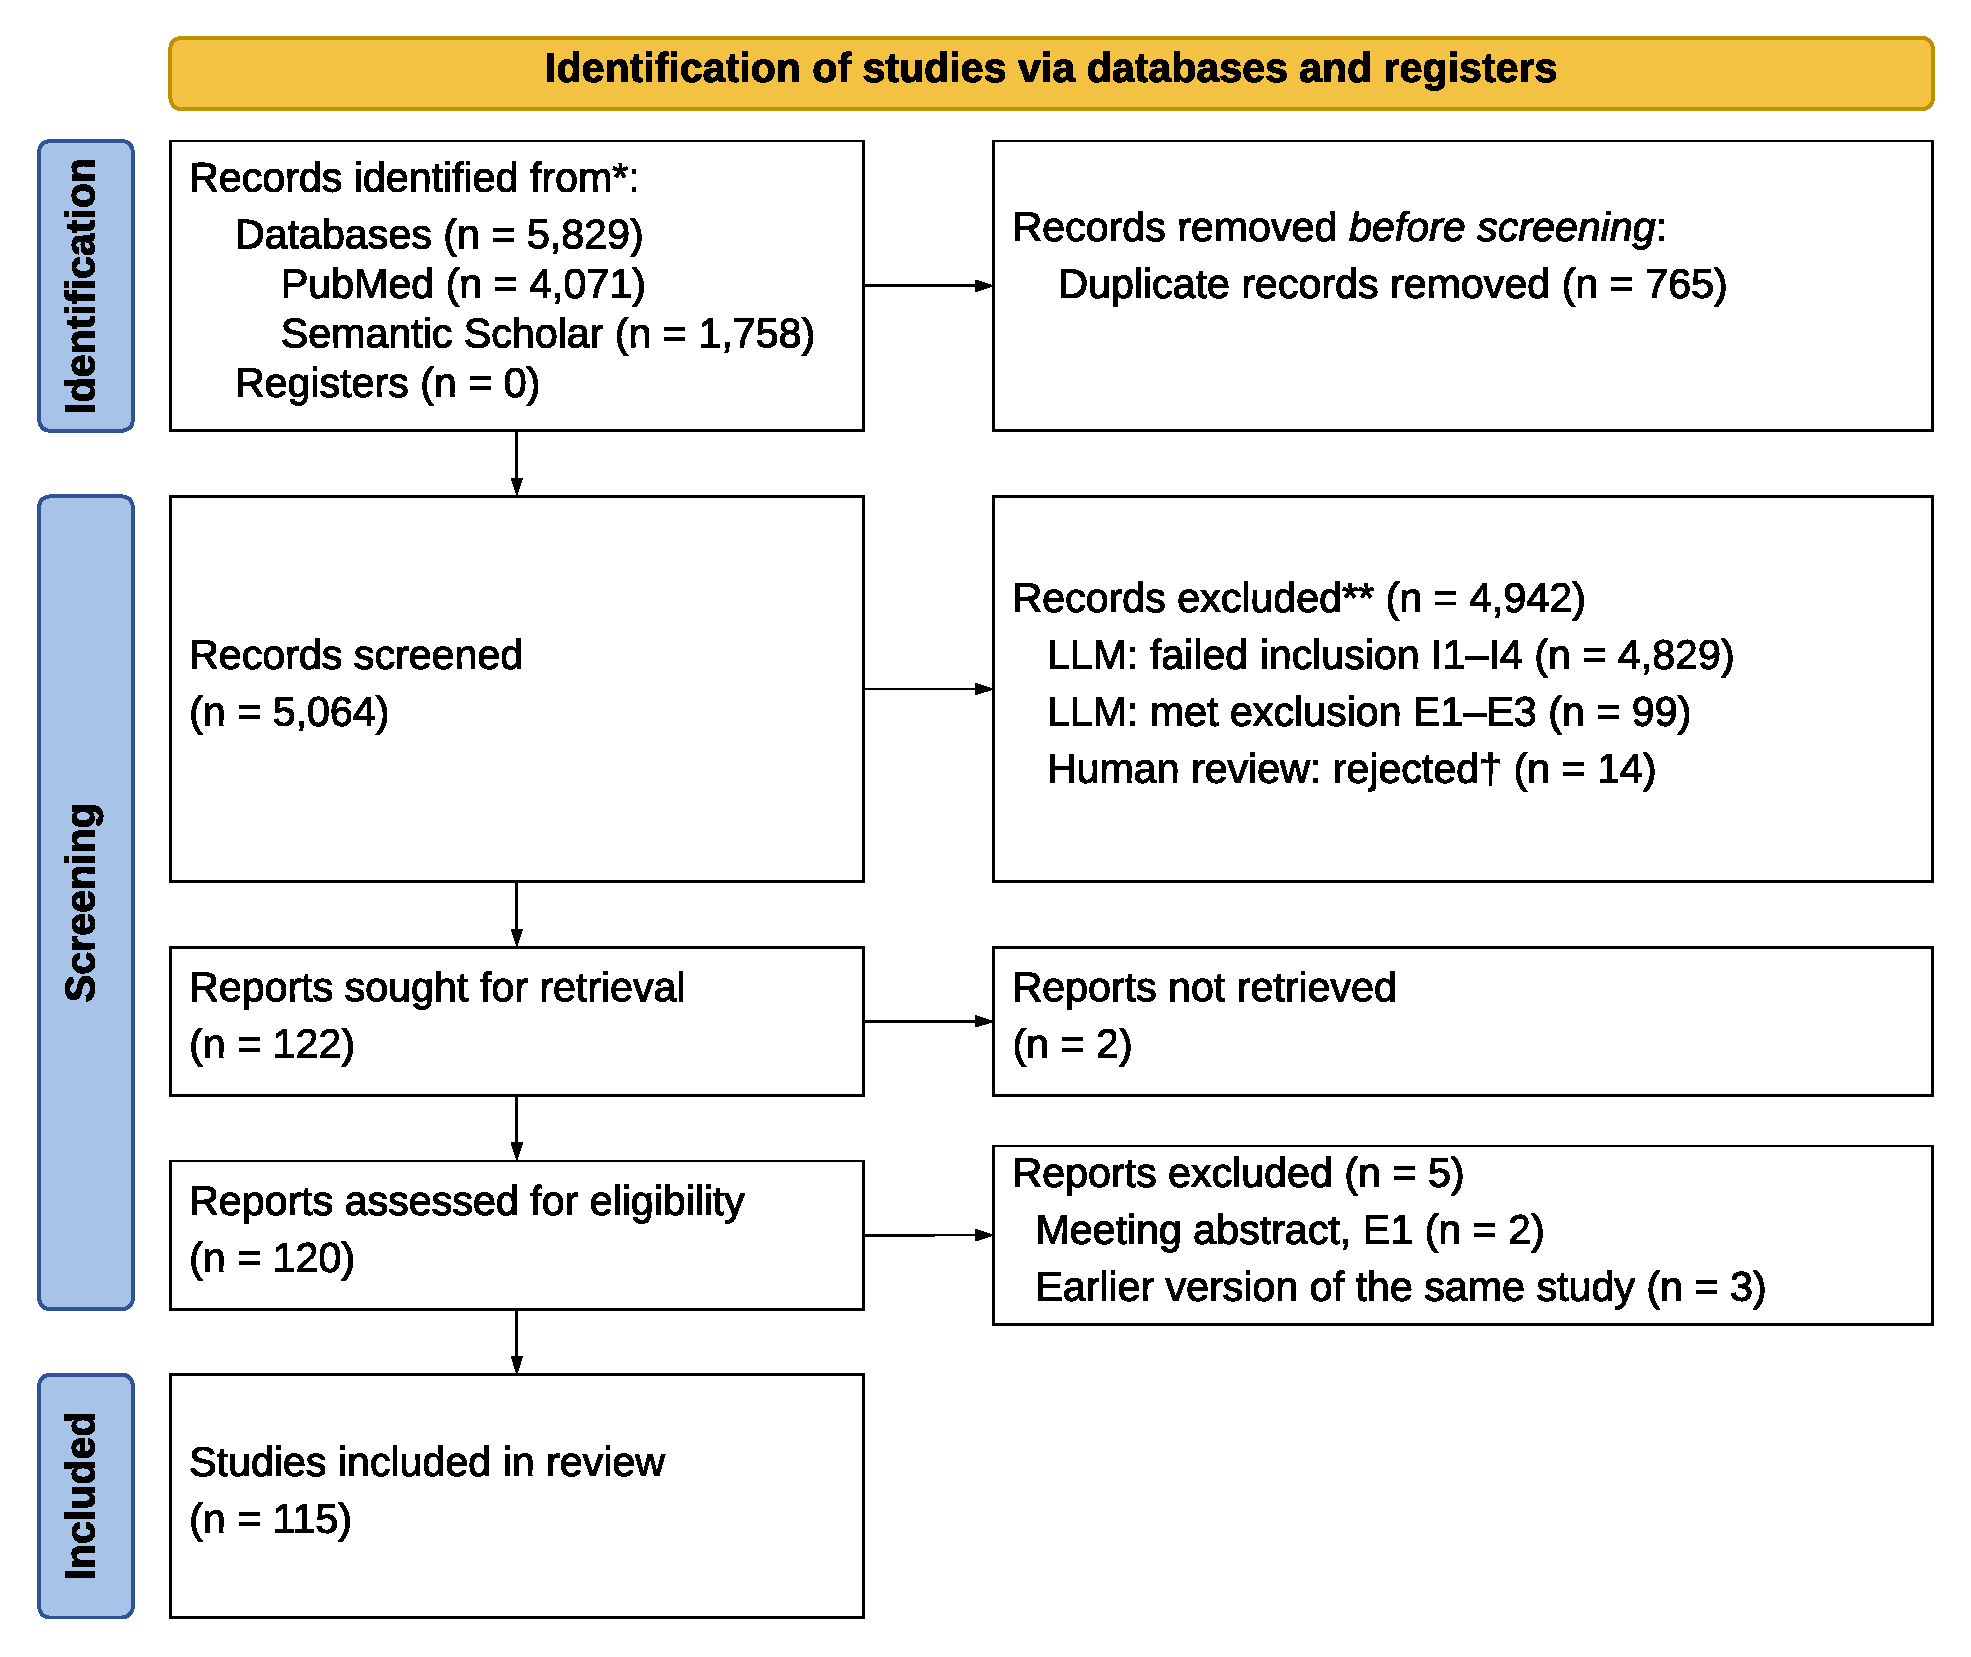
\includegraphics[width=\textwidth, height=13.6cm]{figs/prisma.pdf}
  \caption{PRISMA 2020 flow diagram of study identification, screening, eligibility assessment and inclusion. *PubMed/MEDLINE and Semantic Scholar. **Title/abstract screening by the LLM pipeline (Section~\ref{sec:llm-pipeline}), followed by independent dual human review of all 134 LLM-eligible records and a random sample of 357 LLM-excluded records (Cohen's $\kappa=0.978$; disagreements resolved by discussion, Section~\ref{sec:validation}). $^{\dagger}$LLM-eligible records judged ineligible by the reviewers. Two records excluded by the LLM (both on criterion I2) were judged eligible by the reviewers and are counted among the 122 reports sought for retrieval. Full text could not be retrieved for 2 of the \edit{122. Of the 120 reports assessed, 5 were excluded: 2 meeting abstracts (E1) and 3 earlier versions (preprint or conference paper) of studies already included through their journal article,} so \edit{115} studies were included.}
  \label{fig:prisma}
\end{figure*}



\subsection{Publication Trends}
\label{subsec:trends}
\begin{figure}[pos=!htbp]
\centering
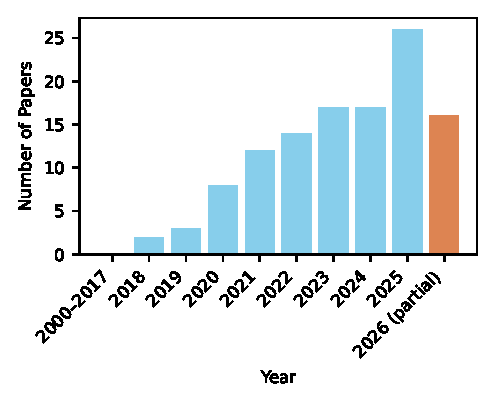
\includegraphics[width=1\linewidth]{figs/temporal_trends.pdf}
\caption{Included studies by publication year. The 2026 bar covers a partial year.}
\label{fig:temporal_trends}
\end{figure}

The trend of the selected articles,  Figure~\ref{fig:temporal_trends}, shows that no included study predates 2018, and only five appeared in 2018--2019. Output rose sharply after 2020 and stayed high through the study inclusion end date. The partial year 2026 already exceeds several earlier full years. 


% Transformer-based temporal models appeared later; all ten such studies were published from 2023 onward.

\vspace{0.25cm}
\begin{mdframed}[linewidth=0.5pt, linecolor=black, backgroundcolor=blue!10]
\textbf{Finding 1.} The field is still growing: 78\% of studies \edit{(90/115)} were published from 2022 to 2026.
\end{mdframed}
\vspace{0.25cm}

\subsection{Imaging Modalities and Anatomical Coverage}
This subsection summarizes the imaging modalities used by the included studies and the anatomical territories they address. The anatomical distribution is shown in Figure~\ref{fig:anatomy_distribution}.


X-ray/fluoroscopy \edit{(55} studies, 48\%) and DSA \edit{(54,} 47\%) are almost equally common, but they are rarely studied jointly: only 5 studies (4\%) use both. Cardiac \edit{(46\%)} and neurologic (41\%) applications, which include cerebral and spinal vascular territories, make up nearly 90\% of the corpus, while abdominopelvic, peripheral, and other thoracic territories are rare (Figure~\ref{fig:anatomy_distribution}). \edit{Most studies develop and test their models within a single territory, so whether} models trained on coronary or cerebral angiography transfer to other vascular regions \edit{remains} \edit{largely} \edit{untested.}

\vspace{0.25cm}
\begin{mdframed}[linewidth=0.5pt, linecolor=black, backgroundcolor=blue!10]
\textbf{Finding 2.} Studies use DSA or X-ray/\allowbreak fluoroscopy in nearly equal numbers but almost never both, and nearly 90\% address cardiac or neurologic territories.
\end{mdframed}
\vspace{0.25cm}






\label{subsec:modality_anatomy}
\begin{figure}[pos=!htbp]
\centering
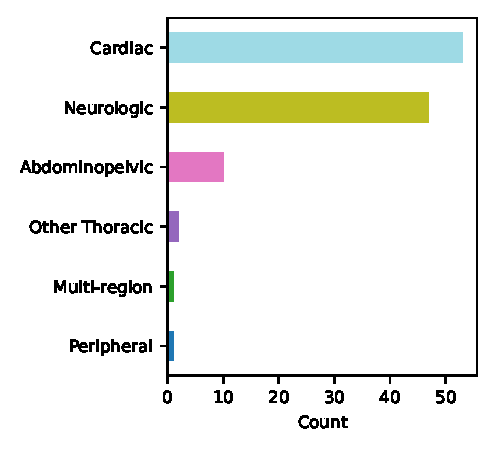
\includegraphics[width=1\linewidth]{figs/anatomy_distribution.pdf}
\caption{Anatomical distribution across included studies. The Neurologic category includes cerebral and spinal vascular territories.}
\label{fig:anatomy_distribution}
\end{figure}


% -----------------

\subsection{Computational Tasks and Model Architectures}
Here, we examined the computational tasks addressed by the included studies and the model architectures used to perform them. We categorized studies by their primary task and summarized the architectures used within each category to characterize the methodological focus of the literature. Figure~\ref{fig:task_distribution} presents the distribution of primary tasks across the \edit{115} studies, while Table~\ref{tab:task_architecture_clean} summarizes the corresponding architectures.
\renewcommand{\arraystretch}{1.25}
\begin{table*}[pos=ht]
\centering
\caption{Temporal-modeling categories of the proposed method in each of the \edit{115} included studies, each assignment backed by a verbatim quote from the article.}
\label{tab:temporal_taxonomy}
\begin{tabularx}{\textwidth}{@{}l X r r@{}}
\toprule
\textbf{Category} & \textbf{Operational Definition} & \textbf{N} & \textbf{\%} \\
\midrule
No Temporal Use
  & Each frame is processed \edit{independently;} no \edit{information} \edit{is} \edit{combined} across frames.
  & \edit{20} & \edit{17.4\%} \\
\dashedrule
Frame Aggregation
  & \edit{Frames} are combined \edit{by} \edit{a} \edit{fixed} \edit{operation} (channel stacking, concatenation, \edit{differencing,} \edit{averaging or temporal pooling)} before a 2D model. \edit{A model trained on stacked frames can learn short-range cross-frame relations, but the sequence has no dedicated temporal mechanism.}
  & \edit{16} & \edit{13.9\%} \\
\dashedrule
Optical Flow / Registration
  & Explicit frame-to-frame motion estimation, registration, or classical tracking/association (e.g., optical flow, particle filters, cross-correlation).
  & 19 & \edit{16.5\%} \\
\dashedrule
RNN / LSTM / GRU
  & Recurrent architectures (LSTM, GRU, ConvLSTM, recurrent residual modules) propagate a hidden state across the sequence.
  & \edit{16} & \edit{13.9\%} \\
\dashedrule
3D CNN / Video Model
  & 3D or spatiotemporal convolutions, or video-/sequence-level representation learning, treating the sequence as a joint spatiotemporal volume.
  & \edit{19} & \edit{16.5\%} \\
\dashedrule
Transformer / State-Space
  & Self-attention or state-space mechanisms modeling long-range dependencies across frames.
  & 10 & \edit{8.7\%} \\
\dashedrule
Hemodynamic / Physics-Informed
  & Explicit physiological or physics-based temporal modeling (reduced-order flow models, hemodynamic priors, time-density curve modeling).
  & 15 & \edit{13.0\%} \\
\midrule
\edit{\textbf{Total}} & & \edit{\textbf{115}} & \edit{\textbf{100.0\%}} \\
\bottomrule
\end{tabularx}
\end{table*}

\renewcommand{\arraystretch}{1.2}
\begin{table}[pos=!htbp]
\centering
\small
\caption{Share of studies using explicit temporal modeling (any category in Table~\ref{tab:temporal_taxonomy} except ``No Temporal \edit{Use'')} by primary task, modality and territory. Rows with fewer than 5 studies are omitted: Background Subtraction (4); Other task (1); Other modality (1); Peripheral (1); Other Thoracic (incl. aortic) (2); Multi-region (1); Not reported (1).}
\label{tab:temporal_crosstab}
\begin{tabularx}{\columnwidth}{@{}X r r@{}}
\toprule
\textbf{Dimension} & \textbf{N} &
\shortstack[r]{\textbf{Temporal-Use}\\\textbf{Rate}} \\
\midrule
\multicolumn{3}{@{}l}{\textit{By Primary Task}} \\
\dashedrule
Temporal Sequence \edit{Modeling} & 6 & 100\% \\
Contrast Flow Analysis & \edit{8} & \edit{100\%} \\
Outcome Prediction & 9 & 89\% \\
Image Enhancement \& Denoising & 9 & 89\% \\
\edit{Vessel} \edit{Segmentation} & \edit{15} & \edit{87\%} \\
\edit{Disease} \edit{Classification} \& \edit{Grading} & \edit{29} & \edit{83\%} \\
Motion Correction \& Registration & 9 & 78\% \\
Object Detection \& \edit{Localization} & \edit{16} & \edit{69\%} \\
Catheter \& Device Tracking & 9 & 67\% \\
\midrule
\multicolumn{3}{@{}l}{\textit{By Imaging Modality}} \\
\dashedrule
DSA & \edit{54} & \edit{87\%} \\
X-ray / Fluoroscopy & \edit{55} & \edit{80\%} \\
DSA + Fluoroscopy (both) & 5 & 60\% \\
\midrule
\multicolumn{3}{@{}l}{\textit{By Anatomical Territory}} \\
\dashedrule
Neurologic & \edit{47} & \edit{91\%} \\
Cardiac & \edit{53} & \edit{79\%} \\
Abdominopelvic & 10 & 60\% \\
\bottomrule
\end{tabularx}
\end{table}
\begin{table*}[pos=t]
\centering
\small
\begin{tabularx}{\textwidth}
{>{\raggedright\arraybackslash}p{4.4cm}
 >{\raggedright\arraybackslash}X}
\toprule
\textbf{Task} & \textbf{Representative Architectures} \\
\midrule

Disease Classification \& Grading (\edit{$n=29$})\newline{\footnotesize\itshape disease label or severity grade} &
CNN classifiers \edit{(16),} recurrent (LSTM/GRU) (5), hybrid CNN--Transformer (3). Examples: DeepRV~\cite{ref198}, ResNet101~\cite{R0099}, X3D~\cite{ref102}, SeqCon~\cite{ref91}, YOLOv8~\cite{R0521}, ResNet-50~\cite{ref161} \\[6pt]

Object Detection \& Localization (\edit{$n=16$})\newline{\footnotesize\itshape locating lesions, stenoses or landmarks} &
object detectors \edit{(9),} hybrid CNN--Transformer \edit{(3), U-Net/encoder--decoder (2).} Examples: YOLOv10x~\cite{R0058}, YOLO Attention~\cite{R0570}, UOA Detector~\cite{ref190}, 2D ResUNet++~\cite{ref20}, 2D convolutional neural network~\cite{R1213}, LT-YOLO~\cite{R1222} \\[6pt]

Vessel Segmentation ($n=15$)\newline{\footnotesize\itshape pixel-wise delineation of vessels} &
U-Net/encoder--decoder (14), hybrid CNN--Transformer (1). Examples: DOSTA-Net~\cite{ref64}, TCA-Net~\cite{ref2}, nnU-Net~\cite{ref15}, TVS-Net~\cite{ref34}, U-Net++~\cite{ref211}, ATFNet~\cite{R1674} \\[6pt]

Catheter \& Device Tracking ($n=9$)\newline{\footnotesize\itshape following devices across frames} &
U-Net/encoder--decoder (5), other learned models (2), hybrid CNN--Transformer (2). Examples: Stent-RD-UNet~\cite{ref178}, Neuro-Vascular Assist~\cite{R1362}, TAG-DL~\cite{ref56}, ConTrack~\cite{R3149}, U-Net~\cite{ref79}, Improved U-Net~\cite{ref162} \\[6pt]

Contrast Flow Analysis (\edit{$n=8$})\newline{\footnotesize\itshape perfusion or flow from contrast} &
CNN classifiers \edit{(3), U-Net/encoder--decoder} (3), other learned models (2). Examples: custom convolutional neural network~\cite{R0100}, perfDSA~\cite{ref28}, YOLOv8m~\cite{R1680}, ResNet~\cite{ref43}, Physics-informed neural network~\cite{R2786} \\[6pt]

Image Enhancement \& Denoising ($n=9$)\newline{\footnotesize\itshape improving image quality or reducing dose} &
other learned models (4), U-Net/encoder--decoder (3), hybrid CNN--Transformer (2). Examples: SAVE-Net~\cite{ref152}, GenDSA~\cite{ref39}, SepConv++~\cite{ref51}, GaraMoSt~\cite{R2490}, MoSt-DSA~\cite{ref104}, ASRNet~\cite{R3126} \\[6pt]

Motion Correction \& Registration ($n=9$)\newline{\footnotesize\itshape aligning frames, views or modalities} &
U-Net/encoder--decoder (4), other learned models (4), non-learning (1). Examples: VGG encoders~\cite{R2400}, Residual U-Net~\cite{ref227}, 4DRGS~\cite{R2466}, TiAVox~\cite{R3164}, SSDR network~\cite{R3338}, RAFT~\cite{ref74} \\[6pt]

Outcome Prediction ($n=9$)\newline{\footnotesize\itshape predicting a clinical outcome or event} &
classical ML (5), other learned models (2), hybrid CNN--Transformer (1). Examples: hybrid transformer-UNet~\cite{ref42}, XGBoost~\cite{ref127}, CLIP ViT-B/32~\cite{R0643}, Deep neural network~\cite{R1263}, logistic regression~\cite{R1503}, gradient boosting classifier~\cite{R1609} \\[6pt]

Temporal Sequence Modeling ($n=6$)\newline{\footnotesize\itshape sequence itself is the output, e.g., phase detection} &
recurrent (LSTM/GRU) (2), CNN classifiers (2), generative (GAN/diffusion) (1). Examples: CDKD-w+~\cite{ref36}, STA-IPCon~\cite{ref57}, Auxiliary Input in Training~\cite{R2411}, ResNet-50~\cite{ref148}, U-Net-like vesselness network~\cite{ref95}, MGR-Net~\cite{ref96} \\[6pt]

Background Subtraction ($n=4$)\newline{\footnotesize\itshape producing DSA-like subtracted images} &
other learned models (1), U-Net/encoder--decoder (1), generative (GAN/diffusion) (1). Examples: HyperMorph~\cite{ref40}, 3D U-Net~\cite{ref52}, pix2pix~\cite{ref93}, rigid registration with mutual information~\cite{R4804} \\[6pt]

Other ($n=1$)\newline{\footnotesize\itshape none of the above} &
other learned models (1). Examples: AngioPlus Core~\cite{R3052} \\[6pt]

\bottomrule
\end{tabularx}
\caption{Architecture families by primary task. Each task is shown with a short definition and $n$, the number of studies; the three most frequent families are listed with study counts, followed by up to six named architectures with the studies that use them.}
\label{tab:task_architecture_clean}
\end{table*}



Figure~\ref{fig:task_distribution} shows that disease classification and grading is the most common primary task \edit{(29} of \edit{115} studies), followed by object detection \& localization \edit{(16)} and vessel segmentation (15). Regarding the model architectures (Table~\ref{tab:task_architecture_clean}) involved in those tasks, 14 of the 15 segmentation studies use encoder--decoder models, mostly U-Net variants; detection studies use YOLO, DETR and R-CNN detectors on ResNet backbones; classification relies on ResNet-style CNNs, with Transformers increasingly added. The majority of architectures are adapted from natural-image computer vision rather than designed specifically for angiography.

Tasks that produce a temporal output remain uncommon. These included temporal sequence modeling, such as cardiac cycle detection and key-frame identification (6 studies), and contrast flow analysis \edit{(8} studies). Many spatial tasks, such as segmentation, detection, and classification, use several frames only to stabilize a per-frame prediction (discussed in detail in Section~\ref{subsec:temporal_taxonomy}).


\label{subsec:tasks_architectures}
\begin{figure*}[pos=!tp]
\centering
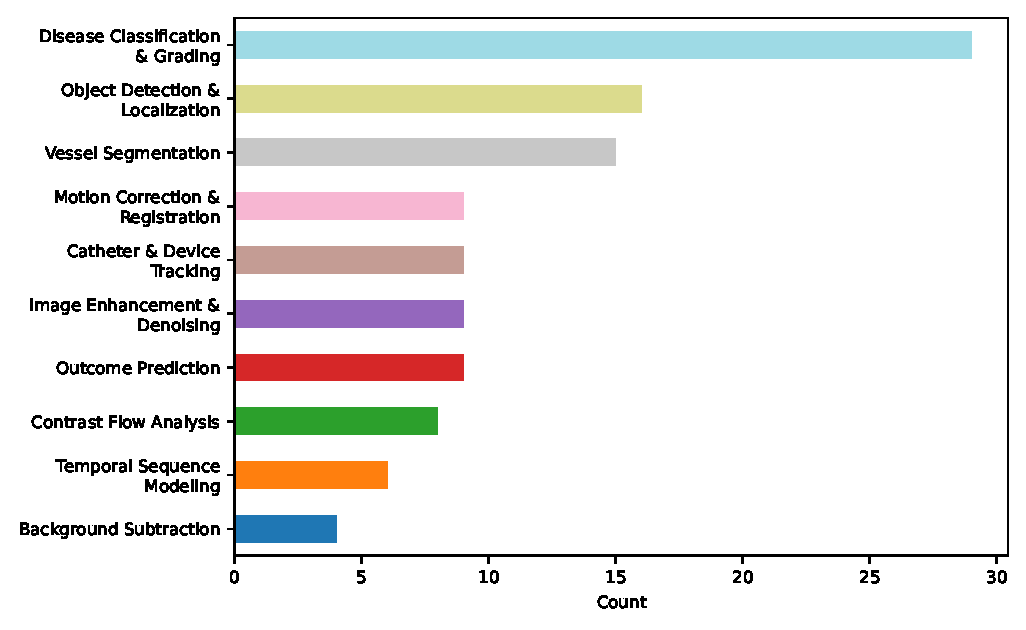
\includegraphics[width=1\linewidth]{figs/task_distribution.pdf}
\caption{Distribution of primary computational tasks across included studies. Task definitions are given in Table~\ref{tab:task_architecture_clean}.}
\label{fig:task_distribution}
\end{figure*}




\subsubsection{Task Category Overlap}
\label{subsec:task_dendrogram}

This subsection examines how often computational task categories occur together within the same study and whether their overlap supports broader task groupings. We compared the sets of studies assigned to each category, considering both primary and secondary tasks, and applied average-linkage clustering to their pairwise Tanimoto \cite{rogers1960tanimoto} distances. Figure~\ref{fig:task_dendrogram} presents the resulting dendrogram, with lower merge distances indicating greater overlap in study membership.

Figure~\ref{fig:task_dendrogram} shows that most task categories merge near the maximum Tanimoto distance, which indicates limited overlap across the literature. \edit{Two} pairs merge at relatively lower distances: contrast flow analysis with outcome \edit{prediction (0.74), and} classification \edit{with} \edit{detection (0.80), which vessel segmentation} and \edit{then} temporal sequence modeling \edit{join} \edit{at 0.90 and 0.92.} These pairings are consistent with workflows in which flow measurements inform outcome \edit{prediction and} detected lesions are subsequently \edit{graded.} They suggest possible groupings for a coarser taxonomy, although the high merge distances overall indicate that even these associations are limited. Image enhancement \& device tracking, as well as motion correction \& background subtraction, connect to the remaining categories only at the highest merge distances.

\begin{figure*}[pos=!tp]
\centering
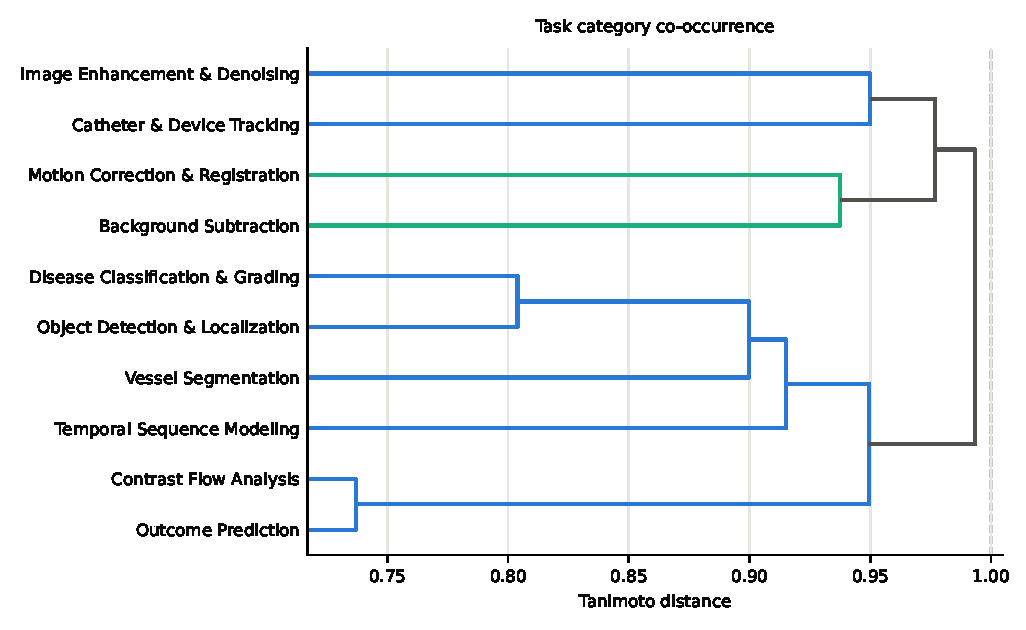
\includegraphics[width=1\linewidth, height=10cm]{figs/task_dendrogram.pdf}
\caption{Average-linkage clustering of ten computational task categories using Tanimoto distances between their study-membership sets, including primary and secondary task assignments. Merges further left indicate greater overlap. All merge distances fall between \edit{0.74} and 1.00; the axis is restricted to this range, and the two sub-clusters with the lowest merge distances are highlighted in color.}
\label{fig:task_dendrogram}
\end{figure*}




\subsubsection{Temporal Modeling}
\label{subsec:temporal_taxonomy}

This subsection examines \edit{how studies use information across frames}. We categorized temporal modeling strategies and compared their use across tasks, imaging modalities, anatomical regions, and publication periods. Table~\ref{tab:temporal_taxonomy} summarizes these strategies and Table~\ref{tab:temporal_crosstab} shows their distribution across study characteristics.

\edit{Ninety-five} of the \edit{115} studies \edit{(82.6\%)} explicitly consider sequential data (linked frames, where a particular visual data instance contains a set of image frames), \edit{and} \edit{20 (17.4\%)} process frames \edit{independently.} \edit{This high proportion partly reflects inclusion criterion I2. The most common} strategies are 3D/video convolution \edit{and} optical flow or registration \edit{(19} \edit{studies each), followed by} recurrent networks \edit{and} frame aggregation \edit{(16 each)} and hemodynamic or physics-based models \edit{(15).} Transformer or state-space models are least common (10 studies, \edit{8.7\%),} all published from 2023 onward. \edit{Frame aggregation is a boundary case: a 2D network trained on stacked frames can learn short-range relations between them, but the sequence has no dedicated temporal mechanism.}

Temporal modeling varies by task, from 100\% for temporal sequence modeling \edit{and contrast flow analysis} to 67\% for catheter and device tracking, Table~\ref{tab:temporal_crosstab}. It is slightly more common in DSA studies \edit{(87\%)} than in X-ray/fluoroscopy studies \edit{(80\%),} and in neurologic studies \edit{(91\%)} than in cardiac \edit{(79\%)} or abdominopelvic studies (60\%). Its prevalence increased substantially over the study period from 40\% in 2018--2019 (2 of 5 studies) to 75--100\% in 2020--2025. In the partial year 2026, it fell to \edit{59\%} (10 of \edit{17} studies).

Of the 95 studies that use sequential frame data, 50 use fixed operations, namely frame aggregation, optical flow or registration, and hemodynamic models. The remaining \edit{45} \edit{(39.1\%} of all studies) learn temporal representations through recurrent, 3D/video, or transformer/state-space models. Learned temporal models are concentrated in disease classification \edit{(20} of \edit{29} studies), absent from image enhancement and device tracking (0 of 9 each), and uncommon in flow analysis \edit{(1 of 8)} and outcome prediction (1 of \edit{9).} Their prevalence increased from \edit{28.2\%} in 2018--2022 \edit{(11} of \edit{39} studies) to \edit{44.7\%} in 2023--2026 \edit{(34} of \edit{76).} Nevertheless, 41 studies \edit{(35.7\%)} use short frame stacks rather than full sequences, and \edit{61 of all 115 studies} identify limited temporal modeling as a limitation.

\vspace{0.25cm}
\begin{mdframed}[linewidth=0.5pt, linecolor=black, backgroundcolor=blue!10]
\textbf{Finding 3.} Although \edit{82.6\%} of studies used sequential frame data, roughly half use fixed temporal operations. Learned temporal representations remain concentrated in classification, while transformer or state-space models appear in only \edit{8.7\%} of studies.
\end{mdframed}
\vspace{0.25cm}





\subsection{Publication Venues}
\label{subsec:venues}

This subsection examines the venues in which the included studies were published. Publication venues indicate which research communities contribute to the field and which journals and proceedings readers need to follow to keep up with it. Figure~\ref{fig:venue_stacked} shows the most frequent venues, while Figure~\ref{fig:venue_curve} shows the cumulative share of studies as venues are added in descending order of publication count.

Of the \edit{115} included studies, \edit{86} \edit{(74.8\%)} were journal articles, \edit{22} \edit{(19.1\%)} were conference papers, and 7 \edit{(6.1\%)} were preprints. Figure~\ref{fig:venue_stacked} shows that the SPIE proceedings are the most frequent outlet, with \edit{10} \edit{studies.} IJCARS and IEEE TMI follow with 5 studies each, and Medical Image Analysis with 4. IEEE venues \edit{and SPIE proceedings each account for 10 studies,} while MICCAI accounts for 3.


% None of the articles appeared in ACM venues; because ACM is a major computing publisher, this suggests that the work is published in imaging and medical venues rather than in general computer-science outlets.

Figure~\ref{fig:venue_curve} \edit{shows how widely the studies are spread across venues.} The \edit{17} most frequent venues account for \edit{half} of the \edit{studies,} \edit{and 50} venues are required to reach 80\%. Of the \edit{72} venues, \edit{54} contribute only one study.

\vspace{0.25cm}
\begin{mdframed}[linewidth=0.5pt, linecolor=black, backgroundcolor=blue!10]
\textbf{Finding 4.} The selected \edit{115} publications are dispersed across \edit{72} venues, \edit{54} of which contribute a single study. Because no venue concentrates this literature, researchers and practitioners seeking to understand the current state of the field must survey a broad range of journals and conference proceedings.
\end{mdframed}
\vspace{0.25cm}

% Figures 7 and 8 share one full-width float so they do not leave half-empty column pages;
% width= sets the cas-dc caption width for each side.
\begin{figure*}[pos=!tp,width=\columnwidth]
\begin{minipage}[t]{\columnwidth}
\centering
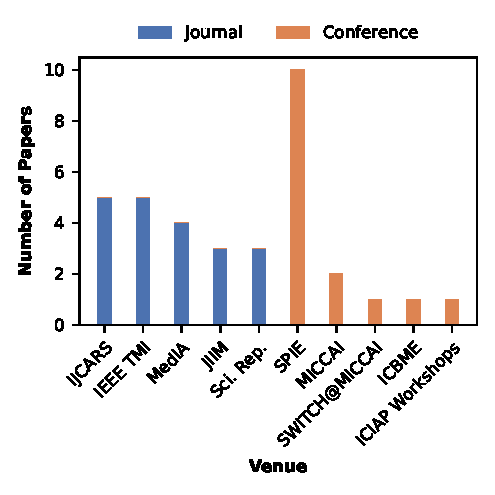
\includegraphics[width=\linewidth]{figs/venue_analysis_stacked.pdf}
\caption{Top publication venues by study count, stratified by venue type. IJCARS: International Journal of Computer Assisted Radiology and Surgery; IEEE TMI: IEEE Transactions on Medical Imaging; MedIA: Medical Image Analysis; JIIM: Journal of Imaging Informatics in Medicine; Sci.\ Rep.: Scientific Reports; SPIE: Proceedings of SPIE; MICCAI: International Conference on Medical Image Computing and Computer-Assisted Intervention; SWITCH@MICCAI: SWITCH workshop at MICCAI; ICBME: Iranian Conference on Biomedical Engineering; \edit{ICIAP} \edit{Workshops: workshops} of the \edit{International} \edit{Conference} \edit{on} \edit{Image} \edit{Analysis} \edit{and} Processing.}
\label{fig:venue_stacked}
\end{minipage}\hfill
\begin{minipage}[t]{\columnwidth}
\centering
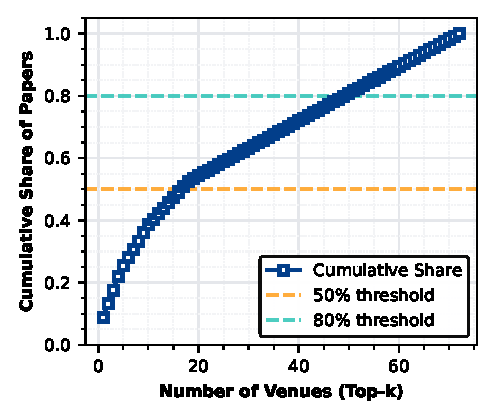
\includegraphics[width=\linewidth]{figs/venue_cumulative_curve.pdf}
\caption{Cumulative share of the \edit{115 studies (one without a stated venue)} across \edit{72} venues, ranked by study count. Dashed lines mark 50\% (yellow) and 80\% (green).}
\label{fig:venue_curve}
\end{minipage}
\end{figure*}


\subsection{Reported Performance}
\label{subsec:performance}

Reported performance metrics are the main basis on which studies compare methods, but each value is meaningful only together with the dataset, validation design, and metric definition that produced it. This subsection examines the reported performance values and their variation across metric families. The values are grouped by metric family and their distributions are shown as a histogram on a scale of 0--100 in Figure~\ref{fig:metric_histogram}. These summaries describe reported results rather than pooled estimates of model performance.

Figure~\ref{fig:metric_histogram} \edit{shows that, within each metric family,} reported scores are concentrated near the upper end of the \edit{scale,} although several studies report substantially lower values. \edit{Taking each study's primary metric, accuracy is reported by 26 studies (mean 86.6, SD 12.0), AUC by 24 (mean 85.7, SD 8.6), Dice/F1 by 14 (mean 87.9, SD 7.5)} and detection precision/recall \edit{by} \edit{10} \edit{(mean} \edit{89.9,} \edit{SD} \edit{12.5);} \edit{IoU} is reported by a single study (75.4). \edit{These families measure different quantities, so we did not average across them.} 

Nonetheless, heterogeneity in datasets, evaluation protocols, and metric definitions precluded direct comparison of performance across studies, and few studies shared a common dataset. A quantitative meta-analysis of reported results was therefore not conducted. Grouping metrics into families does not make them interchangeable, and accuracy alone can obscure poor performance on minority classes. The concentration of high values may reflect selective reporting or testing on data similar to the training data. However, this distribution analysis alone cannot establish either explanation.

\vspace{0.25cm}
\begin{mdframed}[linewidth=0.5pt, linecolor=black, backgroundcolor=blue!10]
\textbf{Finding 5.} Reported performance is generally high, but differences in datasets, protocols, and metrics prevent reliable cross-study rankings in the absence of a shared benchmark.
\end{mdframed}
\vspace{0.25cm}




\begin{figure*}[pos=!tp]
\centering
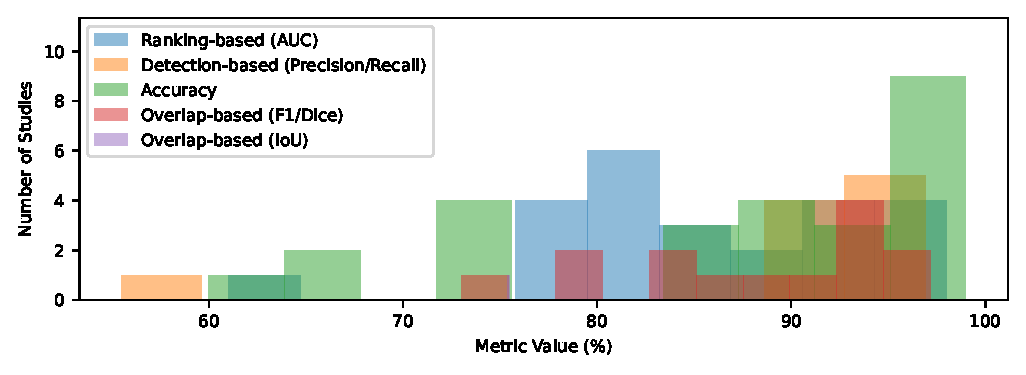
\includegraphics[width=1\linewidth]{figs/histogram_metrics.pdf}
\caption{Distributions of reported performance values by metric family, expressed on a 0--100 scale. Values are descriptive and do not represent pooled performance estimates.}
\label{fig:metric_histogram}
\end{figure*}


% Figure~\ref{fig:metric_kde} provides a smoothed view of these distributions, making their concentration and spread easier to distinguish.

% \begin{figure}[!htbp]
% \centering
% 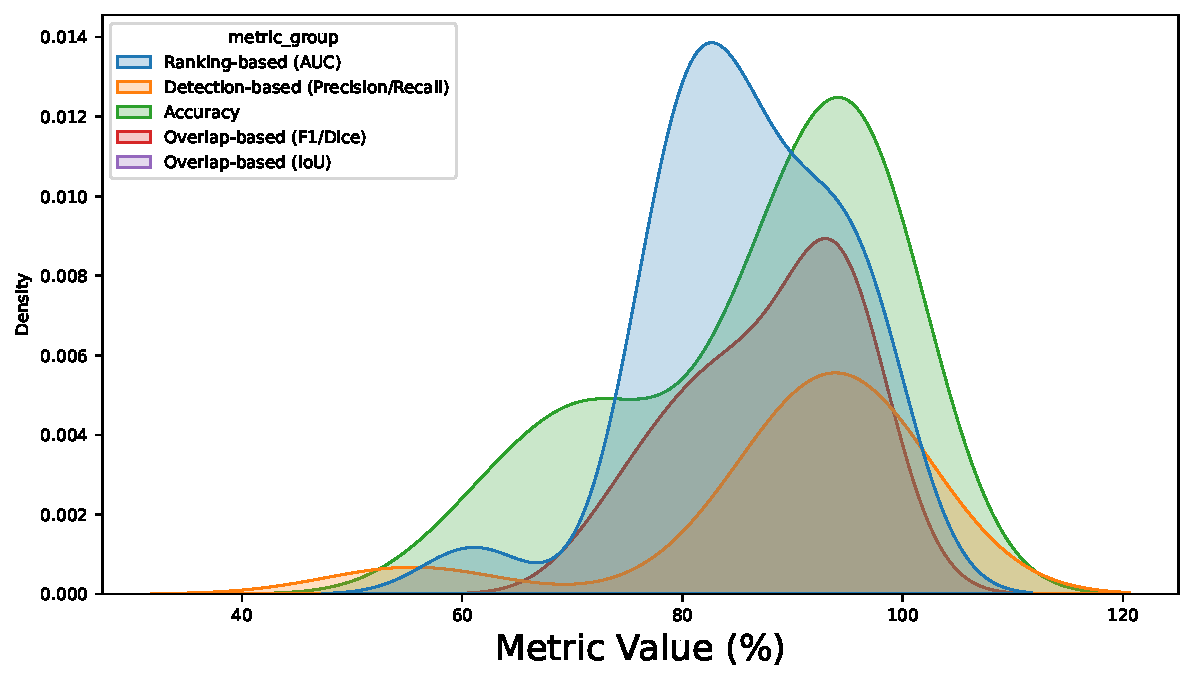
\includegraphics[width=1\linewidth]{figs/kde_metrics.pdf}
% \caption{Kernel density estimates showing smoothed distributions of reported performance values by metric family. Differences in study settings and metric definitions limit direct comparisons.}
% \label{fig:metric_kde}
% \end{figure}




\subsection{Reporting Quality and Clinical Readiness}
\label{subsec:reporting_quality}

We assessed reporting completeness against the 44 items of the CLAIM 2024 checklist~\cite{Tejani2024}, using its official item numbers, and separately summarized evidence supporting clinical \edit{use.} Items are summarized within the 14 subsections of the checklist, from Title and abstract (items 1--2) to Other information (items 42--44), and we compared studies published up to 2024 with those published from 2025 onward as an early check of whether the most recent literature shows any shift toward the updated checklist.


\definecolor{claimTA}{HTML}{4C72B0}
\definecolor{claimIntro}{HTML}{55A868}
\definecolor{claimMeth}{HTML}{C44E52}
\definecolor{claimRes}{HTML}{DD8452}
\definecolor{claimDisc}{HTML}{8172B2}
\definecolor{claimRepro}{HTML}{937860}

\begin{table*}[pos=!tp]
  \centering
  \caption{Reporting completeness by CLAIM 2024 checklist subsection, studies published up to 2024 vs.\ from 2025 onward. The split follows the publication of CLAIM 2024~\cite{Tejani2024}. Items are official CLAIM 2024 item numbers with short descriptions.}
  \label{tab:claim2024_temporal}

  \footnotesize
  \renewcommand{\arraystretch}{1.25}
  \setlength{\tabcolsep}{4pt}

  \resizebox{\textwidth}{!}{%
  \begin{tabular}{@{}
      p{2.6cm}
      c
      p{8.6cm}
      r r
      r r
      >{\centering\arraybackslash}p{1.9cm}
  @{}}

    \toprule

    \multicolumn{1}{l}{\textbf{Subsection}} &
    \multicolumn{1}{c}{\textbf{Items}} &
    \multicolumn{1}{l}{\textbf{CLAIM 2024 checklist items}} &
    \multicolumn{2}{c}{$\boldsymbol{\leq 2024}$ \textbf{(N\,=\,\edit{73})}} &
    \multicolumn{2}{c}{$\boldsymbol{\geq 2025}$ \textbf{(N\,=\,\edit{42})}} &
    \multicolumn{1}{c}{$\boldsymbol{\Delta}$ \textbf{($p$)}} \\

    \cmidrule(lr){4-5}
    \cmidrule(lr){6-7}

    & & &
    \textbf{\%} & \textbf{95\% CI} &
    \textbf{\%} & \textbf{95\% CI} &
    \\

    \midrule

    \rowcolor{claimTA!15}
    \multicolumn{8}{l}{\textbf{\textcolor{claimTA}{Title/Abstract}}} \\

    Title \& abstract & 1--2 & 1 identification as an AI study; 2 structured summary of design, methods, results and conclusions
    & 100\% & [95, 100]
    & 100\% & [92, 100]
    & $\pm0\%$ (1.00) \\

    \midrule
    \rowcolor{claimIntro!15}
    \multicolumn{8}{l}{\textbf{\textcolor{claimIntro}{Introduction}}} \\

     & 3--4 & 3 scientific and clinical background, including the intended role of AI; 4 aims and objectives
    & 100\% & [95, 100]
    & 100\% & [92, 100]
    & $\pm0\%$ (1.00) \\

    \midrule
    \rowcolor{claimMeth!15}
    \multicolumn{8}{l}{\textbf{\textcolor{claimMeth}{Methods}}} \\

    Study design & 5--6 & 5 prospective or retrospective; 6 study goal and intended use
    & 100\% & [95, 100]
    & 100\% & [92, 100]
    & $\pm0\%$ (1.00) \\

    Data & 7--13 & 7 data sources; 8 inclusion and exclusion criteria; 9 data preprocessing; 10 selection of data subsets; 11 de-identification; 12 missing data; 13 image acquisition protocol
    & \edit{59\%} & [47, \edit{70]}
    & \edit{64\%} & \edit{[49,} \edit{77]}
    & $+5\%$ \edit{(0.69)} \\

    Reference standard & 14--18 & 14 definition of the reference standard; 15 rationale for choosing it; 16 source of annotations and annotator qualifications; 17 annotation of the test set; 18 inter- and intrarater variability
    & 76\% & [65, \edit{85]}
    & \edit{69\%} & \edit{[54,} \edit{81]}
    & $-7\%$ \edit{(0.51)} \\

    Data partitions & 19--20 & 19 assignment of data to partitions; 20 level at which partitions are disjoint
    & 84\% & \edit{[74,} \edit{91]}
    & \edit{78\%} & \edit{[63,} \edit{88]}
    & $-6\%$ \edit{(0.45)} \\

    Testing data & 21 & 21 intended sample size
    & 4\% & [1, \edit{12]}
    & 5\% & [1, 16]
    & $+1\%$ (1.00) \\

    Model & 22--24 & 22 detailed model description; 23 software libraries and frameworks; 24 initialization of model parameters
    & \edit{67\%} & \edit{[56,} \edit{77]}
    & \edit{64\%} & \edit{[49,} \edit{77]}
    & $-3\%$ (0.84) \\

    Training & 25--27 & 25 training details (augmentation, objective function, hyperparameters, stopping criteria); 26 selection of the final model; 27 ensembling
    & \edit{54\%} & [42, \edit{65]}
    & \edit{44\%} & \edit{[30,} \edit{59]}
    & $-10\%$ \edit{(0.43)} \\

    Evaluation & 28--34 & 28 performance metrics and comparison with prior models; 29 statistical significance and uncertainty; 30 robustness or sensitivity analysis; 31 explainability; 32 evaluation on internal data; 33 testing on external data; 34 clinical trial registration
    & \edit{59\%} & [47, \edit{70]}
    & \edit{60\%} & \edit{[45,} \edit{73]}
    & \edit{$+1\%$} (1.00) \\

    \midrule
    \rowcolor{claimRes!15}
    \multicolumn{8}{l}{\textbf{\textcolor{claimRes}{Results}}} \\

    Data & 35--36 & 35 numbers of patients or examinations included and excluded; 36 demographic and clinical characteristics
    & \edit{54\%} & \edit{[43,} \edit{65]}
    & \edit{64\%} & \edit{[49,} \edit{77]}
    & $+10\%$ \edit{(0.33)} \\

    Model performance & 37--39 & 37 performance on all partitions and datasets; 38 diagnostic performance estimates with their precision; 39 failure analysis
    & \edit{92\%} & \edit{[83,} 96]
    & \edit{81\%} & \edit{[67,} \edit{90]}
    & $-11\%$ \edit{(0.14)} \\

    \midrule
    \rowcolor{claimDisc!15}
    \multicolumn{8}{l}{\textbf{\textcolor{claimDisc}{Discussion}}} \\

     & 40--41 & 40 limitations; 41 implications for practice
    & 100\% & [95, 100]
    & \edit{98\%} & \edit{[88,} \edit{100]}
    & $-2\%$ \edit{(0.37)} \\

    \midrule
    \rowcolor{claimRepro!15}
    \multicolumn{8}{l}{\textbf{\textcolor{claimRepro}{Other information}}} \\

     & 42--44 & 42 reference to the full protocol or technical details; 43 availability of software, model or data; 44 funding and role of funders
    & \edit{51\%} & \edit{[40,} \edit{62]}
    & \edit{71\%} & \edit{[56,} \edit{83]}
    & $+21\%$ \edit{(0.03)} \\

    \bottomrule

  \end{tabular}%
  }

  \par\smallskip
  \footnotesize
  \textit{Note:} Proportion of studies in which the subsection is reported (at least half of its applicable items), among studies where it applies, with 95\% Wilson CIs. $\Delta$: difference from unrounded proportions, with the two-sided Fisher's exact $p$-value. No subsection is significant after Holm correction (smallest adjusted \edit{$p=0.46$}). Item 34 (clinical trial registration) was not applicable to any study.

\end{table*}
% \definecolor{claimTA}{HTML}{4C72B0}
% \definecolor{claimIntro}{HTML}{55A868}
% \definecolor{claimMeth}{HTML}{C44E52}
% \definecolor{claimRes}{HTML}{DD8452}
% \definecolor{claimDisc}{HTML}{8172B2}
% \definecolor{claimRepro}{HTML}{937860}

% \begin{table}[ht]
%   \centering
%   \caption{CLAIM 2024 Adherence by Thematic Cluster: Temporal Comparison
%     ($\leq 2024$ vs.\ $\geq 2025$).}
%   \label{tab:claim2024_temporal}

%   \footnotesize
%   \renewcommand{\arraystretch}{1.25}
%   \setlength{\tabcolsep}{4pt}

%   \resizebox{\columnwidth}{!}{%
%   \begin{tabular}{@{}
%       l
%       p{6.2cm}
%       r r
%       r r
%       >{\centering\arraybackslash}p{1.2cm}
%   @{}}

%     \toprule

%     \multicolumn{1}{l}{\textbf{ID}} &
%     \multicolumn{1}{l}{\textbf{Cluster}} &
%     \multicolumn{2}{c}{$\boldsymbol{\leq 2024}$ \textbf{(N\,=\,77)}} &
%     \multicolumn{2}{c}{$\boldsymbol{\geq 2025}$ \textbf{(N\,=\,43)}} &
%     \multicolumn{1}{c}{$\boldsymbol{\Delta}$} \\

%     \cmidrule(lr){3-4}
%     \cmidrule(lr){5-6}

%     & &
%     \textbf{\%} & \textbf{95\% CI} &
%     \textbf{\%} & \textbf{95\% CI} &
%     \\

%     \midrule

%     \rowcolor{claimTA!15}
%     \multicolumn{7}{l}{\textbf{\textcolor{claimTA}{Title/Abstract}}} \\

%     C01 & AI identification \& abstract completeness
%     & 71\% & [62, 78]
%     & 75\% & [62, 84]
%     & $+4\%$~$\uparrow$ \\

%     \midrule

%     \rowcolor{claimIntro!15}
%     \multicolumn{7}{l}{\textbf{\textcolor{claimIntro}{Introduction}}} \\

%     C02 & Background \& study objectives
%     & 98\% & [94, 100]
%     & 98\% & [91, 100]
%     & $\pm0\%$~$\sim$ \\

%     \midrule

%     \rowcolor{claimMeth!15}
%     \multicolumn{7}{l}{\textbf{\textcolor{claimMeth}{Methods}}} \\

%     C03 & Study design \& data sources
%     & 42\% & [34, 50]
%     & 61\% & [48, 72]
%     & $+19\%$~$\uparrow$ \\

%     C04 & Participants \& image acquisition
%     & 29\% & [21, 37]
%     & 38\% & [26, 51]
%     & $+9\%$~$\uparrow$ \\

%     C05 & Reference standards \& annotation
%     & 31\% & [24, 40]
%     & 46\% & [34, 59]
%     & $+15\%$~$\uparrow$ \\

%     C06 & Data partitioning \& class handling
%     & 44\% & [36, 53]
%     & 44\% & [31, 57]
%     & $\pm0\%$~$\sim$ \\

%     C07 & Model architecture \& training
%     & 65\% & [56, 72]
%     & 64\% & [50, 75]
%     & $-1\%$~$\sim$ \\

%     C08 & Evaluation design \& interpretability
%     & 24\% & [17, 32]
%     & 52\% & [39, 64]
%     & $+28\%$~$\uparrow$ \\

%     \midrule

%     \rowcolor{claimRes!15}
%     \multicolumn{7}{l}{\textbf{\textcolor{claimRes}{Results}}} \\

%     C09 & Performance \& external validation
%     & 35\% & [27, 44]
%     & 44\% & [31, 57]
%     & $+9\%$~$\uparrow$ \\

%     C10 & Demographic \& subgroup reporting
%     & 8\% & [4, 14]
%     & 16\% & [9, 28]
%     & $+8\%$~$\uparrow$ \\

%     \midrule

%     \rowcolor{claimDisc!15}
%     \multicolumn{7}{l}{\textbf{\textcolor{claimDisc}{Discussion}}} \\

%     C11 & Limitations, implications \& supporting documentation
%     & 84\% & [77, 90]
%     & 89\% & [79, 95]
%     & $+5\%$~$\uparrow$ \\

%     \midrule

%     \rowcolor{claimRepro!15}
%     \multicolumn{7}{l}{\textbf{\textcolor{claimRepro}{Reproducibility \& Transparency}}} \\

%     C12 & Reproducibility \& funding disclosure
%     & 21\% & [15, 29]
%     & 23\% & [14, 36]
%     & $+2\%$~$\sim$ \\

%     \bottomrule

%     \multicolumn{7}{p{\hsize}}{%
%       \textit{Note:} Proportions are the fraction of studies reporting adherence
%       (``Yes'') among those where the item was applicable (NA excluded).
%       95\% Wilson confidence intervals are shown.
%       $\Delta$ = post--pre difference; arrows indicate changes greater than
%       2 percentage points.
%     } \\

%   \end{tabular}%
%   }

% \end{table}


Table~\ref{tab:claim2024_temporal} shows reporting completeness for each checklist subsection with 95\% Wilson confidence intervals and the comparisons between publication periods. The title, abstract, introduction and study design subsections are reported by every study, and the discussion by nearly all. Methods reporting is weaker and less consistent: training details (items 25--27) are reported by \edit{54\%} and \edit{44\%} of studies in the two periods, and the testing-data subsection (item 21, intended sample size) by only 4\% and 5\%. The largest differences between periods are in other information (items 42--44: \edit{51\%} to \edit{71\%,} unadjusted \edit{$p=0.03$}), model performance (items 37--39: \edit{92\%} to \edit{81\%,} $p=0.14$) and results data (items 35--36: \edit{54\%} to \edit{64\%,} $p=0.33$). No difference is statistically significant after Holm correction (smallest adjusted \edit{$p=0.46$}).

\edit{At the item level, reporting rates were calculated across all 115 studies, with nonapplicable items counted as not reported. Test-set size justification was the least reported item (item 21: 5 studies, 4.3\%), followed by external testing (item 33: 19, 16.5\%) and inter-rater variability (item 18: 23, 20.0\%). Other infrequently reported items were explainability (item 31: 26, 22.6\%), de-identification (item 11: 27, 23.5\%), complete training details (item 25: 29, 25.2\%), statistical uncertainty (item 29: 30, 26.1\%) and handling of missing data (item 12: 31, 27.0\%). Demographic and clinical characteristics were reported by 48 studies (item 36: 41.7\%). Low reporting rates across all studies sometimes reflected limited applicability: ensembling (item 27) was reported by 10 of the 11 studies that used ensembles. Trial registration (item 34) did not apply to any study because none was a clinical trial.}




Although 52 studies \edit{(45.2\%)} include a statement on the availability of software, models or data (item 43), only 25 studies \edit{(21.7\%)} publicly release code and 3 \edit{(2.6\%)} publicly release their own data. We counted a release only when the article gave a working repository or archive link; statements that data are available on reasonable request, made by \edit{26} further studies, were not counted. An availability statement does not necessarily indicate public release, because many such statements restrict access. Evidence supporting clinical use was also limited: 19 studies \edit{(16.5\%)} report external validation, including one that also reports prospective deployment; 3 \edit{(2.6\%)} use a prospective design; 4 \edit{(3.5\%)} report clinical deployment or live use; and 4 \edit{(3.5\%)} discuss regulatory requirements. These categories are not mutually exclusive.

\vspace{0.25cm}
\begin{mdframed}[linewidth=0.5pt, linecolor=black, backgroundcolor=blue!10]
\textbf{Finding 6.} Against the CLAIM 2024 checklist, title, abstract, introduction and study design are well reported, but test-set size justification, external testing, inter-rater variability, training details, statistical uncertainty, demographic characteristics, code and data sharing, and evidence of clinical use remain limited. We found no statistically significant difference in reporting in studies published prior to, and after, the CLAIM-2024 publication.
\end{mdframed}
\vspace{0.25cm}

